% !TEX program = xelatex
\documentclass[UTF8,a4paper,zihao=-4,fontset=fandol]{ctexart}
\usepackage[left=25mm,right=25mm,top=25mm,bottom=25mm,headheight=15pt]{geometry}
\usepackage{amsmath,amssymb,booktabs,tabularx,longtable,array,graphicx}
\usepackage{caption,fancyhdr,enumitem,needspace,xurl,hyperref}
\usepackage{tikz}
\usetikzlibrary{arrows.meta,positioning}
\hypersetup{unicode=true,colorlinks=true,linkcolor=black,citecolor=black,urlcolor=black,
  pdftitle={Lab-ultra-unified：面向数学建模论文的双路论文蒸馏与可追溯数模工作流},
  pdfauthor={Lab-ultra-unified 项目设计说明},pdfsubject={架构、信息流、写作蒸馏、科学绘图与验证边界}}
\setlength{\parindent}{2em}
\setlength{\parskip}{0pt}
\linespread{1.16}
\setlength{\emergencystretch}{2em}
\clubpenalty=10000
\widowpenalty=10000
\displaywidowpenalty=10000
\ctexset{section={format=\Large\bfseries,beforeskip=1.1em,afterskip=.6em},
  subsection={format=\large\bfseries,beforeskip=.8em,afterskip=.4em}}
\captionsetup{font=small,labelfont=bf,labelsep=quad,skip=7pt}
\setlist{nosep,leftmargin=2em}
\pagestyle{fancy}\fancyhf{}
\fancyhead[L]{\small Lab-ultra-unified：论文蒸馏与工作流}
\fancyhead[R]{\small 技术设计论文}
\fancyfoot[C]{\small\thepage}
\renewcommand{\headrulewidth}{.3pt}
\newcolumntype{Y}{>{\raggedright\arraybackslash}X}
\newcommand{\sys}{\textsf{Lab-ultra-unified}}
\newcommand{\code}[1]{\texttt{\small #1}}
\title{\bfseries Lab-ultra-unified：面向数学建模论文的\\双路论文蒸馏与可追溯数模工作流}
\author{项目设计与实现说明（统一版）}
\date{2026 年 9 月 13 日}

\begin{document}
\maketitle
\begin{abstract}
数学建模论文需要同时保持模型解释、计算结果、图文组织与版本修订的一致性。本文介绍 Lab-ultra-unified，一套由一个协调入口与十九个子模块组成的论文工作流，并详细说明其离线蒸馏与运行时使用方式。系统将论文资料分为版式与内容两条处理路线：版式路线由确定性解析器提取页面几何，以结构语义组织统计，通过按篇加权、代表样式选取及分组验证研究可迁移的排版控制；内容路线从连续文本中建立论证地图，提取带原文定位的表达动作，经引用校验、语义复核和条件归并形成写作资源。2026 年 9 月 10 日统一版基于 1,585 份最终文本分析，为 6,230 条原候选建立采用或排除去向，另吸收 46 条补充记录，得到 68 个通用技巧与 145 个条件细分。运行时按具体读者困难检索规则，保留适用条件及误用限制，利用轻量证据依赖记录连接计算、正文、图注和审查。本文在原有设计论文基础上更新版本与实现说明，加入统一技巧库的数据结构、版式准入边界、完整分发机制和药材烘干论文案例。已有发行记录包含 20 模块、265 个资源文件及 128 项通过的回归检查；本次另外复核了资源哈希与写作查询。上述证据支持已记录的接口和局部表达行为，尚不足以确认整篇论文质量的统计提升。

\end{abstract}
\noindent\textbf{关键词：}数学建模；Skill；内容蒸馏；语义版式；条件写作技巧；证据溯源

\section{引言}

数学建模论文的困难不只在于求出一个数值结果。作者需要把现实对象转化为数学关系，说明简化为何成立，选择能够检验关键判断的计算方式，再把结果组织为读者可以独立理解和检查的论证。对智能体而言，这些环节还有额外的协调成本：变量可能在代码与正文中含义不同，一项更正可能只更新结果表而未进入摘要，精美的示意图可能暗示并不存在的物理机制，编译成功的 PDF 也可能保留已经失效的结论。

方法资料、运行脚本和写作指南各有用途，但它们需要围绕同一个问题协作。模型选择要能够接回现实对象，求解记录要能定位到实际输出，章节整合要处理共享符号与条件，排版则应保留已经确认的内容。\sys{} 把这些接口作为主要实现对象，使模型可以自由选择方法，同时让成果的来源和适用范围能够被查阅。

系统的任务环境专门化主要通过 Skill 指令、结构化参考资源和确定性工具完成。本文使用“蒸馏”指从来源材料提取、核查并归并可迁移经验的过程。内容蒸馏没有训练或发布新的基础大模型权重；版式研究则包括统计建模和有边界的参数投影。二者的输出和验证责任不同，因此分别介绍。

本文绑定的运行时版本是 \code{lab-ultra-unified-20260910-r2}，文稿修订日期为 2026 年 9 月 13 日。对外项目名为 \code{lab-ultra-unified}，实际调用入口仍是 \code{lab-ultra}，同套子模块使用 \code{lab-ultra-*}。维护源位于实验目录的 \code{candidate/skills/}；旧 lab-pro、labv3 和稳定版 cumcm 保持各自身份。正文中的当前实现均以该统一版的文件与 manifest 为准\cite{install}。

本文的设计工作集中在两处。其一，把语料中的页面安排和解释动作分别转化为可检查的数据，避免两类证据混用；其二，将归并后的规则接入按需写作和版本追踪，使来源经验能够在具体解释困难处被调用。文中同时保留设计意图、实现事实、历史试验与本次核查的区别。

\section{任务范围与设计目标}

\subsection{任务环境的专门化与方法选择的开放性}

\sys{} 面向的是中国数模国赛的任务环境，而不是所有科研任务的无差别自动化。题目通常由多个问题和附件构成，要求作者在限定条件下给出模型、计算结果和可解释的方案。领域专门化因此主要体现在附件语义、跨问联系、假设说明、符号约定、论文表达和交付边界上，而不是把每一类赛题绑定到固定算法。

主入口先识别用户要求的操作范围。审计已有结论、实现指定模型、润色一段文字和完成整道题，需要的权限与工作量不同。对只读审计，系统不进入实现；对固定模型计算，发现模型限制后应报告问题，而不能为了方便求解而偷偷替换公式；对局部润色，也不因为文本属于论文就自动启动文献检索、绘图和全篇排版。

若将一次任务的可执行动作集合记为 $\mathcal A$，用户授权记为 $U$，已知证据及其适用范围记为 $E$，可用工具与资源预算记为 $R$，则系统希望保留的决策空间可写为
\begin{equation}
\mathcal A_{\mathrm{allowed}}=\{a\in\mathcal A:\ a\text{ 满足 }U,\ a\text{ 不歪曲 }E,\ a\text{ 不超出 }R\}.
\label{eq:autonomy}
\end{equation}
式\eqref{eq:autonomy}是设计原则的形式化概括，不是当前实现中的自动规划求解器。“不歪曲证据”并不禁止提出新假设，而是要求将假设与事实分开；资源约束也不规定固定候选数量，只要求有意义的探索在授权范围内进行。

\subsection{硬边界、表达引导与可选资料}

系统把约束分为不同性质的三层。第一层是不能靠审美偏好抵消的边界，例如不得伪造结果、不得改变被锁定的数学含义、不得把未审查状态报告为通过。第二层是必要的任务引导，例如在重要公式附近说明对象、条件与后果，在跨问承接处说明什么成为下一问的输入，在摘要中保留改变结论范围的限定。第三层是按需检索的范例、工具说明和条件技巧。第三层不应覆盖第一层，也不应让第二层膨胀成每段必须满足的格式表。

这一区分回应了自主性与控制之间的表面矛盾。精确控制可以放在可核验的成果接口上，而不必侵入每一步推理。系统不设置统一的创新数量、模型比较数量、图表配额或摘要句数。方法简单并不意味着贡献不足，采用库外方法也不自动构成创新；判断依据是该方法是否回答问题，以及相应主张是否得到支持。

\section{总体架构：一个协调入口与按需展开的能力集合}

\subsection{二十模块的职责划分}

\sys{} 采用一个主协调模块与十九个子模块。表\ref{tab:modules}按责任将二十个模块归为三个层次，而非将其解释为二十个必须依次执行的阶段。主协调模块维护任务范围、共享证据和未决问题；领域模块承担建模、计算和写作等操作；图形模块内部再根据图意和工具能力选择专门路线。

\begin{table}[htbp]
\centering\small
\caption{完整套件的职责划分。模块名省略共同的 \texttt{lab-ultra-} 前缀；主入口为 \texttt{lab-ultra}。}
\label{tab:modules}
\begin{tabularx}{\linewidth}{@{}p{24mm}Yp{12mm}Y@{}}
\toprule
层次 & 模块 & 数量 & 主要责任\\
\midrule
主协调 & lab-ultra & 1 & 确认范围、按需分派、整合结果与安排复核\\
建模与论文 & intake、modeling、compute、writing、review、references、sciverse、typesetter & 8 & 题意与资料、数学构造、真实计算、正文、审查、检索和排版\\
科学图形 & scientific-figure-maker、academic-plotting、agent-figure-gallery、draw-io、evaluate-diagram、figure-generation、figure-spec、generate-diagram、generate-plot、scientific-visualization、scipilot-figure-skill & 11 & 图意组织、参考检索、图形生成、导出和检查\\
\bottomrule
\end{tabularx}
\end{table}

模块数量不是能力强弱的量度。保留已有成熟工具的目的，是复用实现、资产及可编辑格式，而不是把它们逐个展示给用户。主协调层只提供操作入口，具体规则留在负责该事项的模块中。普通写作不需要预载全部检索库；单幅图形也不需要同时使用所有图形子模块。由此形成的按需展开机制，旨在减少无关指令对当前任务的干扰，但其上下文效率仍需通过同任务对照测量，不能仅由文件组织推定。

\subsection{离线维护与运行时的连接}

离线侧保存来源清单、解析结果、审读记录、候选归并与布局研究；运行时侧保存经过整理的技巧、策略、脚本及必要参考。普通写作只查询相关规则，排版也不重新遍历语料库。图\ref{fig:architecture}给出两侧的产物流向，框中的对象是数据或职责，不能据此推定已经启动相同数量的智能体。

\begin{figure}[htbp]
\centering
\begin{tikzpicture}[box/.style={draw=black!60,rounded corners=1pt,align=center,font=\small,text width=55mm,minimum height=12mm,inner sep=5pt},arr/.style={-{Stealth[length=2mm]},thick},node distance=9mm]
\node[box] (src) {来源登记与解析\\原文、版本、坐标、角色};
\node[box,below=12mm of src,xshift=-40mm] (lay) {版式分析\\LayoutIR、语义、按篇统计};
\node[box,below=12mm of src,xshift=40mm] (con) {内容分析\\论证地图、候选、原文定位};
\node[box,below=of lay] (policy) {版式策略\\有限参数、来源及准入状态};
\node[box,below=of con] (cards) {统一写作资源\\68 个通用技巧、145 个细分};
\node[box,below=42mm of src,text width=48mm,yshift=-23mm] (run) {运行时协调\\计算、写作、图形与排版};
\node[box,below=of run] (out) {正文、图表、可编辑文件\\证据版本与检查记录};
\draw[arr] (src)--(lay);\draw[arr] (src)--(con);
\draw[arr] (lay)--(policy);\draw[arr] (con)--(cards);
\draw[arr] (policy.south)--(run.west);\draw[arr] (cards.south)--(run.east);
\draw[arr] (run)--(out);
\end{tikzpicture}
\caption{离线双路蒸馏与运行时的产物流向。版式研究结果只有在满足相应检查或保持明确的既有选择身份时进入运行时；候选分析需经过采用决定才能成为写作规则。}
\label{fig:architecture}
\end{figure}

这种分离也决定了发布内容。安装包中的来源定位可以指出开发分析记录，但不意味着原始论文、OCR 全文及所有研究日志均已打包。维护者更新技巧时回到原始证据，普通使用者则从已经整理的条件规则入手。对于依赖外部服务的检索和图形能力，宿主仍需要相应连接与运行环境。

\subsection{Skill 与 worker 的区别}

Skill 是可复用的操作知识，worker 是一次实际执行任务的智能体。读取两个 Skill，不等于已经启动两个 worker；在文档里写出“建模专家”和“审稿专家”，也不构成协同证据。\sys{} 因而同时保留单智能体执行与宿主原生协作两种方式：小范围、自包含的任务由当前智能体完成；可独立推进的实质工作和重要的非作者审阅，才适合委派。

协作的价值需要由独立产物或检查体现。对于整篇论文，主协调者仍对最终答案负责，写作模块或指定编辑者负责正文整合，计算者负责数值结果，图形者负责科学编码与图像，排版者负责页面组织。多个 worker 不应同时写同一个可变文件；委派章节需要携带该节在全篇中的作用、相邻语境、共享符号、材料版本和不可更改的条件。这样才能避免接回四段分别完整、拼在一起却重复和矛盾的文字。

\subsection{对 Danus 思想的选择性吸收}

Danus 公开项目把数学研究中的任务组织、事实关系和验证职责显式化，并包含从论证材料到论文的写作环节\cite{danus}。\sys{} 吸收的是材料精选、依赖关系、成稿复核和范文学习的思想，而非直接部署其完整运行时。项目记录明确说明，本地适配没有整体复制其服务、数据库或权限模型\cite{integration}。

这种取舍源于任务差异。数模探索中存在观测误差、经验模型、近似算法和解释性主张，不能把所有材料压缩成同一种“已证明事实”。\sys{} 因此使用包含事实、假设、计算、解释和限制的证据关系，而不把版本工具解释成真理数据库；采用宿主已经提供的智能体能力，而不另设常驻调度服务。协作是为解决工作分离和复核问题服务的，不是每次任务都要经过的仪式。

\section{信息流：让结果、解释和修订指向同一份证据}

\subsection{一项主张需要的不只是一个数值}

计算交接常见的失败是只传递“误差下降了”或一张结果表。写作者随后不得不猜测比较分母、样本范围、训练与测试划分，以及误差对应的物理单位。\sys{} 要求重要计算结果携带输入和代码版本、实际输出、单位、执行记录以及与主张相关的诊断。执行记录说明程序运行过，但收敛状态、可行性、独立验证或数值误差仍需分别判断。

系统不为每种证据强造运行回执。解析推导有其前提与推理，外部文献有其版本与定位，给定事实有其题目出处。计算工具只负责自己能够记录的过程。这种证据类型的分离，使“程序退出成功”“数值合理”和“论文结论成立”不会在交接时被合并成一个含糊的通过状态。

\subsection{选择性的证据依赖图}

当一项结果影响多个章节、图注或审查记录时，系统提供可选的轻量依赖图。记
\begin{equation}
G=(V,E_{\mathrm d},E_{\mathrm q}),
\label{eq:graph}
\end{equation}
其中，$V$ 为证据、主张、图形、正文与审阅等节点；$E_{\mathrm d}$ 为使用上游材料的依赖边；$E_{\mathrm q}$ 为必须随主张共同阅读的限定或不利证据边。后一类关系不是正向支持。例如，设备留出实验可能限制随机划分结果的适用范围，不能只因它不支持正文的乐观判断就从阅读材料中删除。

每个节点保存稳定标识、摘要、适用范围、来源定位、文件哈希与声明依赖。当前工具实现了创建快照、检查绑定、选取相关材料和预览变化影响四类操作\cite{coordinator}。对发生变化的节点集合 $C$，需要重新检查的已声明范围可概括为
\begin{equation}
\mathcal I(C)=C\cup\operatorname{Desc}_{E_{\mathrm d}\cup E_{\mathrm q}}(C),
\label{eq:impact}
\end{equation}
其中边按“上游材料指向消费者”的方向理解，$\operatorname{Desc}$ 表示沿两类关系可到达的下游节点。式\eqref{eq:impact}描述的是声明关系上的影响范围，而非自动发现全文全部依赖的算法。未声明的关系不会因此获得独立性保证；依赖覆盖不足时，审阅者需要扩大检查。

版本新鲜并不等于内容正确。文件哈希一致，只能说明目前读取的是曾经绑定的字节；错误论证也可以拥有完全一致的哈希。反过来，过期状态表示旧审查不能直接用于新版本，而不表示旧结论必然错误。系统据此避免将证据图变成形式证明器，也不要求每句话、每个临时变量都建成节点。

\subsection{从更正到新成稿的闭环}

有效修订应同时处理事实变化和它的表达后果。例如，一项误差从 $1.8$ 更正为 $2.1$，不只需要替换正文数字，还可能改变相对改善幅度、比较结论、图注、摘要和原审阅的适用性。写作编辑者应读取更正来源，调整受影响的表述，保存新产物，并把新正文与实际审阅记录登记到后继快照。查询旧图中的影响范围，不能替代注册新成稿。

独立审阅从两个方向进行：一是由来源判断它实际支持什么，二是由成稿判断读者会理解成什么。两者不完全相同。数字逐项正确的摘要，仍可能因为省略样本条件而形成错误的推广。审阅反馈因此需要定位到具体段落、关系和后果，而不只是给出“逻辑较弱”的评分。修复后复核新版本及其受影响使用处；没有实际审阅时，应明确保留待审状态。

\section{内容蒸馏：从来源文本到条件写作库}

\subsection{来源身份、连续覆盖与未完成材料}

内容路线的输入包括论文、题面、教师评述和其他写作资料。来源登记记录文件哈希、转换文本身份及角色，不把目录中的“获奖”字样直接当作作品认证。同一篇文章的多个 OCR 版本、附件和混排摘要需要建立对应关系，避免重复计算独立支持。来源中的命令、程序与角色说明始终是分析对象，不是蒸馏任务的执行指令\cite{fulltext,api}。

已完成 API 批次的分母为 1,585 份登记转换文本。该数值表示文本分析单元，既不等于 1,585 篇独立获奖论文，也不覆盖整个原始资料库。未转换文件、归档中未解码内容以及未转录媒体继续保留在缺口清单中。早期 64 篇获奖展示稿专项审读与后续全转换文本批次是不同记录口径，不能直接相加。

长文处理采用连续字符分块。设转换文本为 $x$，长度为 $L$，各块区间为 $[a_k,b_k)$，则覆盖检查要求
\begin{equation}
a_1=0,\qquad b_k=a_{k+1},\qquad b_K=L,\qquad
x=x[a_1:b_1]\Vert\cdots\Vert x[a_K:b_K].
\label{eq:coverage}
\end{equation}
其中 $\Vert$ 表示拼接，区间以转换文本的字符位置计。分块尽量在换行处结束，超长单行仍保持连续覆盖；每块携带原文行号。式\eqref{eq:coverage}检查送入任务的范围，不能判断 OCR 是否漏掉原页公式，也不能证明模型理解了每段文字。

\subsection{map、reduce 与 audit 的任务组织}

map 阶段针对收到的文本生成身份判断、论证地图与局部表达候选。论证地图需要说明关键对象和推进关系，不能只列章节标题。reduce 阶段汇总分块结果，并继承已有证据定位；audit 阶段回查表达候选及来源。SQLite 保存文档和任务状态，执行器记录并发、重试和预算预留，哈希用于绑定输入与响应\cite{api}。

候选数据模式见表\ref{tab:move-schema}。每个候选必须说明作者具体做了什么，以及这个动作怎样帮助理解。例如，“使用有限元方法”只描述工具；“先画出受力和约束位置，再说明离散方程中对应项的来源”才包含可迁移的表达关系。

\begin{table}[htbp]
\centering\small
\caption{内容候选的主要字段及校验责任。}
\label{tab:move-schema}
\begin{tabularx}{\linewidth}{@{}p{32mm}YY@{}}
\toprule
字段 & 保存的内容 & 检查重点\\\midrule
\code{start/end} & 原文起止行号 & 位于声明区间及实际输入块内\\
\code{quote} & 对应原文短引文 & 连续文本匹配，不能拼造出处\\
\code{observation} & 作者的具体表达动作 & 回读上下文，区别作者与评述者\\
\code{reader\_benefit} & 解决的理解困难 & 是否能从原段说明该作用\\
\code{transfer} & 可迁移的写法 & 是否仍是表达动作，是否误成算法处方\\
\code{limits} & 条件、缺陷和反例 & 是否保留影响适用性的限定\\
\bottomrule
\end{tabularx}
\end{table}

文档级报告还保存 \code{argument\_map}、\code{roles}、\code{do\_not\_inherit} 与 \code{unresolved}。没有适用经验时允许空候选；公式损坏或缺少图像时留下待核项。引用检查验证文字确实出现在给定区间，reduce 还检查证据是否来自上游结果。通过这些机械条件后，候选仍需要语义复核。

该批次共完成 3,875 个任务，最终失败数为零。其中 1,473 份文本完成全文二次机器复核；112 份长文完成所有分块处理后，只对选取的证据范围进行二次复核。后者不能写成全文二次审读。API 响应截断、角色混淆和来源区间错位均有历史纠正记录，原报告与后继更正保留各自身份\cite{fulltext}。

\subsection{语义归并与逐项去向}

统一版对全部最终分析中的候选建立去向。记原候选集合为 $M$，分析字段和历史复盘补充为 $S$，采用集合与排除集合分别为 $A$、$X$，则本轮登记满足
\begin{equation}
M\cup S=A\,\dot\cup\,X,\qquad
|M|=6230,\ |S|=46,\ |A|=6214,\ |X|=62.
\label{eq:disposition}
\end{equation}
式中 $\dot\cup$ 表示不相交并集。原候选中 6,168 条被吸收，62 条有明确排除理由；46 条补充全部采用。它们是审读输入的处置计数，不是基础模型训练样本数或独立来源篇数。最终产物为 68 个通用技巧与 145 个条件细分\cite{unification}。

归并依据是表达动作和适用条件。相同动作来自不同资料时可以合到共同父类；条件不同的用法继续保留，例如先给直觉再定义适用于读者缺少对象认识的段落，先给定义再讨论适用于容易产生概念歧义的段落。两种经验不需要按来源数量投票淘汰其中之一。暂时分类困难、内容常见或与已有规则同义，都不是排除候选的充分理由。

排除项包括行政提交规范、纯算法操作、没有写作动作的记录，以及会诱导夸大或空泛修辞的建议。具有表达价值但科学主张可疑的来源，可以只迁移经过核对的组织动作。例如保留“分别说明训练误差和外部验证”的写法，不继承“拟合优度足以证明预测可靠”的结论。78 份没有 moves 的分析也纳入其他字段审读，不能因候选为空而跳过整份材料。

第二轮统一记录包含 API 初审、三路原生模型归并及主代理的排除复查和措辞修订。这里的三路是当时的执行记录，不是每次写作必须启动的固定团队。全部 6,230 条原候选均有去向，也不意味着未转换原件已经完成处理。

\subsection{父技巧、条件细分与来源链}

运行时通过 \code{exposition-cards.json} 保存通用技巧，\code{render\_techniques.py} 从该数据生成可读指南；\code{technique-variants.json} 保存条件规则及成员来源。主入口、Markdown 视图与结构化细分共同构成一套写作能力，不另维护相互竞争的指令副本\cite{writing,query}。

一个细分规则包含 \code{id}、\code{card\_id}、\code{rule}、\code{conditions}、\code{misuse}，并关联来源及复核信息。来源可记录 \code{source\_id}、原分析路径、哈希、字段名、行号或定位说明；成员 ID 将归并后的规则连接回原候选。哈希支持检查字节是否变化，不能替代对该来源是否支持规则的判断。

以实际条目 \code{variant-0039} 为例，父技巧是“搜索覆盖与停止理由”。规则要求报告搜索实际覆盖区域、已有界或可行性证据和停止点；条件是有限搜索或迭代的覆盖与停止可记录；误用说明指出，一次稳定或局部搜索不能写成全域最优。原候选可以保留更长的表达与限制，但运行时采用的内容由归并规则明确给出。

这一结构允许维护者修正规则而保留来源历史，也允许使用者只读取当前段落需要的少量信息。源记录中的候选文字只是证据，不能绕过采用决定直接成为执行指令。

\subsection{冲突处置与失败经验}

多个来源出现矛盾时，先比较对象、时间、分母、条件和证据层级。相容的条件分支分别保存；无法核实的命题继续待定。例如人工核验子样本的通过率与全部候选的系统准确率具有不同分母，即使两处数字相同也不能合并。旧分析被原文纠正后，旧记录留作历史，不能继续与新记录共同投票\cite{conflicts}。

早期专项审读曾出现只做机械装载和摘录却申报全文完成的输出；相关记录被拒收后重新审读。该经验促使检查更重视连续区间、具体来源及角色边界。结构完整的 JSON、覆盖旗标和顺畅的总结都不能单独证明完成了内容理解。失败记录因此也是蒸馏过程的产物，用于识别下一轮需要回查的位置。

\section{写作引导与论证组织}

\subsection{从工作顺序转向理解顺序}

程序通常按数据读取、预处理、求解、保存结果的顺序运行，但论文不必按同样的顺序叙述。读者需要先知道哪些对象和区别决定问题，再理解关键关系如何成立，最后判断结果意味着什么。\sys{} 的写作指南据此强调现实对象、数学表达、证据和结论之间的连接\cite{writing}。

例如，“采用非线性最小二乘估计参数”只报告了求解方式。更有解释力的表述应说明：候选参数如何生成观测预测，预测如何与同一条件下的实测值构成残差，哪些参数在多组观测间共享，哪些量随条件变化。这些说明补齐了参数、观测和目标函数之间被省略的关系。此例仅说明写作动作，不表示本文执行过相应拟合。

段落可以承担定义、选择理由、推导、证据比较或适用范围限定等功能，但不必将每段填入预设槽位。模型可以压缩读者已知的材料，并展开决定结论的一步。多问之间若确有依赖，应说明上一问输出怎样进入下一问；若问题彼此独立，则不为了故事完整而编造递进关系。写作的整体感来自共用对象与真实接口，不来自重复的过渡套话。

\subsection{符号体系是一种语义接口}

一致的字形不足以构成一致的符号体系。观测量、潜在状态、决策变量、估计方法和估计值可能都被写作同一个字母；时间下标和迭代下标也可能在不同章节中被混用。\sys{} 要求在重要位置明确符号的对象、作用域、类型、索引、单位和参数来源，而不是仅在开头放置一张大符号表。

以 $y_{ij}$ 与 $\widehat y_{ij}$ 为例，二者若分别表示第 $i$ 个对象在第 $j$ 次观测中的测量值和预测值，就需要说明 $i$、$j$ 的取值范围，以及重复观测是否独立。图轴、结果表、代码列名和正文中的误差都应回到同一对象。物理量及其数值单位必须保持一致，字符串编号不应按测量值进行舍入。变量与单位采用不同字形的通行规范可以辅助阅读\cite{nist}，但字形规范不能代替这些语义定义。

正文解释、公式精确性和符号表各有责任。符号表帮助查阅，公式承载可检查的关系，邻近文字说明该关系为什么适用以及接下来推出什么。一个没有解释建模假设的符号表，并不会因收录完整而补齐论证。

\subsection{按读者困难选择规则}

写作开始时，先识别当前段落缺少的关系：对象没有定义、推导跨步、结果缺少比较口径，或结论超出证据范围。默认指南提醒作者检查这些基本关系，条件库则提供更具体的选择。使用者不需要在每次写作时加载 6,230 条原候选。

查询工具 \code{query\_variants.py} 按规则文字和父技巧 ID 做字面匹配，默认最多返回三条，可用 \code{--card} 限定父技巧。\code{show} 读取确切细分，\code{source} 读取确切候选的来源，\code{health} 检查结构及绑定。工具没有嵌入向量检索或基于大模型的排序，未命中时正常写作，不强制选择无关规则。

检索到规则后，作者把 \code{rule}、\code{conditions}、\code{misuse} 一起应用于已有材料。例如，规则可以帮助说明已经做过的网格检查；如果研究从未执行该检查，不能为了套用规则而补写结果。规则提出的是解释责任，新增计算仍属于另一项工作。

本次在发行资源上执行 \code{health} 与“搜索”查询，确认 68 个父技巧、145 个唯一细分及 \code{variant-0039} 的实际返回。该检查验证了这条检索路径；规则能否改善某一篇完整论文，还取决于任务材料、使用时机和实际改稿结果。

\subsection{先准备资料，后针对问题检索}

资料准备与任务时检索是两个不同过程。前者可广泛收集、去重、筛选并记录版本与使用边界；后者应围绕一个具体知识缺口选取必要片段。当前本地参考模块使用经过整理的双语元数据进行词法检索，不应被描述为覆盖全部论文的语义搜索引擎。需要实时文献时，可经已有 SciVerse 连接查询原始来源，但检索命中仍不等于完成验证。

必要写作引导不能全部藏在一个“有需要再搜索”的库里，否则模型可能根本意识不到需要补充解释。\sys{} 因此把对象到公式、选择到后果、跨问接口、符号区分和摘要保真放在默认指南，把细分技巧留在可直接访问的条件卡中。默认指南提供注意方向，条件库提供可迁移经验；两者都不规定本题必须选用哪一种数学方法。

\section{版式蒸馏：几何测量、结构语义与运行时投影}

\subsection{测量与语义标注分工}

版式路线由 \code{layout-lab} 及共同几何重测工具承担。原生 PDF 通过确定性解析提取页、块、行与 span 的位置、字体、字号、基线和阅读顺序；扫描来源先转换为 OCR 文本与文字框。\code{LayoutIR} 保存这些几何及解析诊断，语义提供者在明确的本体和字段约束下标注角色、关系及置信度\cite{architecture,layoutcal}。

模型收到已有的结构化文字与测量，不负责从语言描述估算坐标或字号。请求和响应保存模型身份、输入哈希、提示词版本及校验结果。缺失块、重复块、无法识别的字段或不一致的模型身份应留下未决状态；规范化记录也要保留。原生几何与 OCR 几何具有不同精度，OCR 行高像素不能直接换算成可靠的正文字号。

\subsection{三个空间与模板混杂}

记语义描述为 $S$、可控排版参数为 $\Theta$、布局质量指标为 $Q$。$S$ 可包含多轴角色和语义关系；$\Theta$ 是有限的 Style Token 集合；$Q$ 包括密度、留白和其他布局诊断。三者的区别在于，内容标签描述文本，控制参数影响渲染，质量指标用于观察结果。把三者直接压成单个审美分数，会掩盖哪些参数实际受到证据支持。

同一期刊模板可能让所有定义和正文采用相近字体。若不控制模板差异，就可能把“定义具有某类语义”误认为导致字体变化的原因。因此研究在同文、同角色内比较语义条件，并采用按论文分组的验证；同时保留已知期刊或出版者的留出结果。抽样语义块不能代替完整页面的几何统计，缺少完整语义覆盖的页面也不能据此给出全页角色占比。

这些统计产生的是样本条件下的观察与候选控制。默认策略仍需受中文段落规范、可读性以及内容和格式检查约束；某个统计中位数本身没有“最佳版式”的含义。

\subsection{按篇加权与国赛优先的共同几何}

获奖展示稿与期刊发现语料在任务、语言、分栏和来源质量上不同。本轮共同几何校准分别给 64 篇国赛稿与 752 个期刊身份分配总质量 $\alpha=0.60$ 和 $1-\alpha=0.40$，组内每篇的权重为
\begin{equation}
w_i=\begin{cases}\alpha/64,& i\in\mathcal C_{\mathrm{award}},\\
(1-\alpha)/752,&i\in\mathcal C_{\mathrm{journal}}.
\end{cases}
\label{eq:weights}
\end{equation}
这种处理防止期刊仅凭篇数优势主导混合统计。$\alpha$ 是面向国赛任务的设计偏好；0.50、0.60、0.70、0.80 的敏感性检查用于观察其影响，不能把 0.60 解释为已经验证的最优权重。

共同重测使用归一化坐标及相同文字筛选，测量文本外包络面积和左右文本边界。设每篇有效几何向量为 $\boldsymbol z_i$，其加权 L1 代表可写为
\begin{equation}
i^\star\in\arg\min_{i\in\mathcal O}\sum_{j\in\mathcal O}
w_j\lVert\boldsymbol z_i-\boldsymbol z_j\rVert_1,
\label{eq:medoid}
\end{equation}
其中 $\mathcal O$ 为该比较所需特征可用的观测集合。代表必须对应实际样本，不能将几种边际均值拼成一篇未出现过的“理想论文”；特征缺失身份和缺失质量另行报告。

国赛特征覆盖为 64/64，期刊为 750/752。$\alpha=0.60$ 时，外包络面积加权中位数为 0.5108075，左右文本边界比例为 0.112 和 0.115；逐年留出的面积中位数约在 0.5053 至 0.5237 之间。medoid 身份会随留出变化。外包络并非文字墨迹面积或文字框并集，边界比例也不能直接作为 LaTeX 页边距\cite{layoutcal}。

\subsection{来源准入与当前默认样式}

752 个期刊身份构成发现语料，只有 21 个具有 \code{publisher-final} 来源锚点资格。v2.1 研究没有得到满足当前导出条件的新共同因子或语义效应。混合校准仍保存 \code{runtime\_transfer\_eligible=false}。这些记录允许研究继续比较假设，不能据此宣布已经完成认证的顶刊版式学习\cite{architecture,layout}。

当前默认投影为 \code{journal-dense-cn-v1}。作者已明确选择该样式，其证据状态仍记录为 \code{legacy\_unverified\_v1}。它是可复现的既有投影，不自动继承后续研究的资格。已明确选择的表题居中作为作者偏好单独记录，也不改写成新学习因子。若配置缺失、无效或不适用，排版应报告原因，按已有授权处理备选样式，不能静默替换。

新策略的导出需要绑定研究产物、准入因子、控制边界与相应选择记录。编译失败、内容改变、缺图、溢出等硬问题独立检查，不能用审美分数补偿。运行时只应用已提供的资源，不重新训练偏好模型或读取整库论文。

\section{科学绘图与排版：分别处理图意、几何和页面}

\subsection{三种图形承担不同的说明责任}

数据图回答数量变化、比较和不确定性问题；机制与几何示意解释对象、约束和关系；三维物理场景则帮助读者识别装置、部件、空间摆放、遮挡和层结构。它们不能相互替代。统计曲线未必能解释观测如何形成，流程方框也不能替代一个具有接触关系的真实场景。

绘图入口因此先确定科学目的、对象与关系，再决定媒介。数据标记必须由实际数据和确定性代码生成；节点与边能够准确表达依赖时可使用 FigureSpec 或 draw.io；几何、公式和局部构型可使用原生 SVG 或 TikZ；需要实体、相机和空间关系时可使用 Blender 或已有 CAD、网格工具。工具选择服从解释保真与现有环境，不以软件专业程度作为质量认证，也不要求安装全部可选工具。

写作者只提出图意时，不需要先构造完整图形协议。真正开始渲染后，图形模块才使用 FigureRequest 和 FigureIR 记录最终尺寸、数据来源、编码、标注、风格及导出目标。统计数据与纯几何输入分开描述；未知物理尺寸可以用明确标识的示意比例呈现，却不能伪装成测量结果。图\ref{fig:scene}展示了本项目的一项已执行路线验证。

\begin{figure}[htbp]
\centering
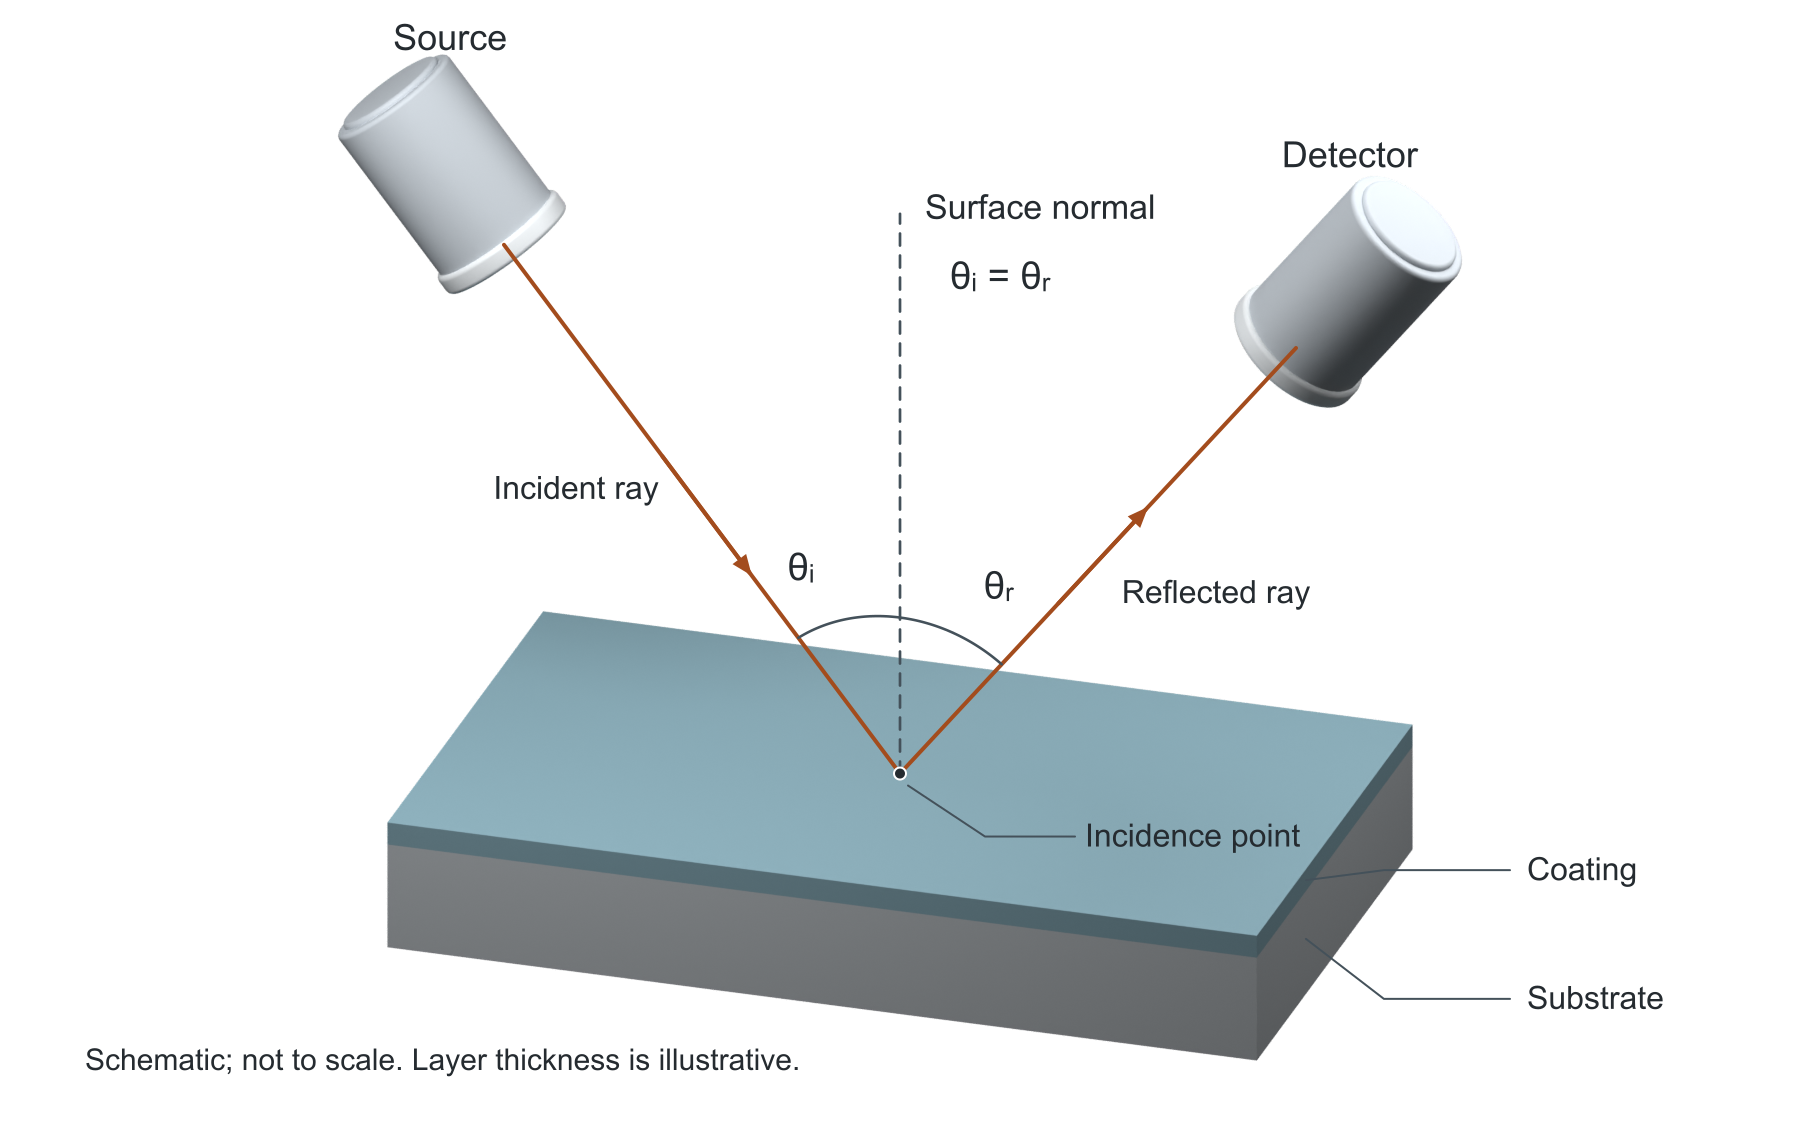
\includegraphics[width=.90\linewidth]{assets/optical-apparatus.png}
\caption{已执行的三维光学装置示意。圆柱体表示简化光源与探测器，蓝灰表层与灰色基体区分材料层，光线和法线的标注由同一相机投影定位。图为合成示意，所有尺寸、层厚及外壳比例均非实测；没有模拟光强或材料响应。此图证明了一条真实几何渲染路线可执行，不证明写作者会在所有论文中自主选择正确的图意。}
\label{fig:scene}
\end{figure}

\subsection{“去 AI 味”应转化为可定位的问题}

本项目观察到的流程图缺陷，并非只由某一种工具产生。一份实际论文直接用 Matplotlib 绘制多组浅色圆角框，且请求的中文字体最终在 PDF 中嵌入为 Black 字重。虽然使用了科研绘图样式辅助函数，最终仍出现拥挤、文字越框和箭头连接不清等问题\cite{physical}。这说明通用样式名称不能替代对实际图像的检查。

系统将相应经验转化为跨工具的图形约束：普通状态默认采用中性文字与克制线条，不自动逐节点轮换颜色；颜色用于区分有意义的对象或条件；中文标签检查实际字面与字重，不只检查字体名称；标签过密时重组信息和布局，而不是无限缩小字号。Nature 的图形指南也强调可读、可编辑的文字及避免多余装饰\cite{nature}，但其具体英文版式指标不直接等同于中文国赛要求。

这种约束不是宣布圆角、彩色或衬线字体一律不科学。表示终止状态的圆角、区分材料的填充以及用户明确指定的字体仍可能合理。真正需要拒绝的是没有解释功能的装饰，以及装饰遮盖的关系错误。控制样式的对照实验中，即使颜色和字体被修正，原图仍可能因为节点内容和连接不当而不合格。

\subsection{排版交付的保真责任}

排版层接收已完成的内容，通过 Pandoc AST、Lua Filter 和 LaTeX 资源组织页面。必要的语法归一、编号和交叉引用可以改变表达载体，公式含义、数字、结论和图表对应关系仍需保持。输出包括可编辑 LaTeX、PDF、输入内容绑定、构建报告及布局审计。

表格分页需要测量实际高度，不能只按行数决定是否跨页。长表保留重复表头、续表标识和脚注；字号不能因挤不下而无限缩小。嵌入图中文字也应在最终 PDF 中检查，正文 CJK 字体正常不意味着图中的中文标签正常。

当前机器报告的通过范围主要是机械检查。生成预览图片不等于已经查看图片，检查全部页码也不证明模型科学有效。视觉审阅应绑定实际 PDF 哈希和查看页码；正文若因实质修订变化，旧的内容审查也需要重新判断适用性。

本文采用独立的中文 LaTeX 技术论文版式，作为系统介绍而非国赛提交稿。其页面质量不计入 \code{journal-dense-cn-v1} 的效果测试，也不据此证明语料研究的新策略已经准入。

\section{实现与验证：哪些环节已经得到证据支持}

\subsection{完整分发与命名空间绑定}

统一版从维护源的明确清单构建 20 个模块，映射主入口及全部子模块名称，同步相对引用和资源哈希。\code{manifest.json} 保存目标文件与源树身份，安装器 \code{install\_lab.py} 完整复制并核验资源，遇到已有同名目录时拒绝合并覆盖。它没有把原始论文、账户认证、外部运行环境或模型权重加入运行时包。

2026 年 9 月 10 日发行记录包含 20 个模块、265 个资源文件和 28 处跨模块入口链接。包内与实际安装后分别通过 128 项回归，失败、错误和跳过均为零；这些重复验证不相加为 256 项不同测试\cite{install,checks}。本次文稿修订重新核对了 265 个文件与安装器哈希，并实际执行写作库健康检查及检索，没有重跑该历史 128 项回归。

更新旧统一版时需要保留原整套模块及对应 manifest，再完整安装新版本。维护源和分发包承担不同责任：前者用于修改与构建，后者用于安装已确定的资源。不应递归搜集仓库中所有 SKILL.md 组成安装包，也不应从旧 lab-pro、labv3 或 vendor 目录拼接模块。

\subsection{版本检查与协作行为试验}

预检工具的早期版本只绑定正文，无法仅凭报告区分正文未变而图像已变的情况。后续实现将正文、解析结构、直接引用图像、检查选项、检查器代码以及 Python 和 Pandoc 版本纳入输入绑定。此改动提升了报告复用条件的可核验性，但仍不覆盖原生 TeX 引用、字体、外部 SVG 资源及完整参考文献依赖\cite{native}。

2026 年 9 月 7 日的合成修订试验提供了前序协作机制的证据，本次未重新执行。材料把方法 A 的平均绝对误差由 $1.8\,\mathrm{nm}$ 更正为 $2.1\,\mathrm{nm}$，方法 B 为 $2.4\,\mathrm{nm}$。在同一台仪器、四十个试样及同一留出划分的限定下，新差值为 $0.3\,\mathrm{nm}$，相对 B 的下降为 $12.5\%$。实际 worker 更新了结果、讨论和摘要，保留无置信区间、无显著性检验和无外部验证等限制，调用非作者审阅者，并将新正文与实际审阅登记到七节点后继快照\cite{native}。这是构造材料上的信息流验证，不是真实设备实验结果。

这次试验没有触发审阅后的再次修复轮次，因此它证明了更正传播、实际委派和后继版本登记，而不是多轮争议处理已经充分验证。另一个局部润色试验中，智能体只修改指定段落，没有启动子智能体、检索或排版。这一结果支持范围控制在该案例中有效，也不等同于润色质量普遍优于基线。

\begin{table}[htbp]
\centering\small
\caption{现有证据的层次与不可外推的结论。不同层次不能相互替代。}
\label{tab:evidence}
\begin{tabularx}{\linewidth}{@{}p{25mm}YY@{}}
\toprule
证据层次 & 已有观察 & 不能据此声称\\
\midrule
分发与回归 & 统一版二十模块、二百六十五文件；发行记录一百二十八项回归通过 & 科学结论或论文写作全部正确\\
条件技巧迁移 & 六个固定事实短段落对照，候选两案轻微偏好、基线一案、三案平手 & 整篇写作稳定提升、达到顶刊水平\\
实际协作 & 合成更正进入结果、讨论、摘要及后继快照，调用非作者审阅 & 真实整篇论文、多作者并发与多轮纠错已充分验收\\
物理场景 & 实际 Blender 渲染、几何关系检查和可编辑标注 & 装置经过工程验证、写作者会自动选对所有图意\\
排版策略 & 历史投影可加载；新统计保留研究与准入边界 & 全量再蒸馏已经成为运行时新共识\\
\bottomrule
\end{tabularx}
\end{table}

\subsection{图形执行与表达比较的结果}

图\ref{fig:scene}所示场景由独立 worker 根据合成光学装置说明生成，保留 Blender 场景、Python 生成器和带可编辑文字及线条的 SVG。其检查记录包含反射方向、等角关系和层间接触，且渲染后实际调整过裁切、标注和几何关系\cite{physical}。SVG 中的实体图像仍是栅格层，不能因外层为 SVG 就称其完全矢量可编辑；实体的编辑能力来自原生场景和生成脚本。

前序表达比较不等同于统一版独立效果评估。六个固定事实案例的短段落对照中，候选版在两案获得轻微偏好，基线在一案获得轻微偏好，三案平手\cite{transfer}。部分关键解释动作在基线中已经存在，候选也仍出现压缩测量条件造成歧义的情况。因此，这些开发案例更适合用于发现规则是否造成误解和过度模板化，而不足以支持长期、稳定的写作收益估计。

\subsection{统一写作库的三个固定证据案例}

统一版的前向核验实际调用条件检索，处理三个受限改稿任务\cite{forward}。第一案给定 20 组参数组合，最后三次计算目标值稳定；改稿保留这些事实，将“全局最优”改为本次搜索范围和终止记录下的稳定。第二案给定 1,000 个候选，其中人工核验 20 个、15 个通过；改稿将 75\% 明确写为已核验子样本通过率 $15/20$，不推广为全部候选的系统准确率。第三案保留交通水流类比及缺少机制验证的事实，把类比定位为解释辅助。

这三个案例检查了规则查询与结论边界的连接，没有新增实验、算法或数值结果。由于它们是限定事实的功能核验，不能由三个案例估计完整论文质量的提升比例，也不能把模型审阅称为人工同行评议。

\section{药材烘干论文：统一工作流的成果展示}

\subsection{案例身份与可观察内容}

作者提供的《圆柱药材烘干的二维热湿传递建模与收缩一致性分析》共 285 页，包含正文与大量源码附录\cite{drying}。本文选择它展示对象定义、方程、离散说明和结果解释如何出现在同一篇成稿中。该成果经历建模及修订，未将其认定为本发行版一次调用的独立基准，也不具有获奖或工程验证标签。

论文以圆柱药材为对象，说明侧面与端面的热质交换，再将温度和含水率场写入二维轴对称模型。在空间离散部分，节点控制体、共享面通量与旋转后的环形体积相互对应，见图\ref{fig:drying-method}。图中对象与附近公式共用符号，读者可以据此检查“一个面流出，邻接单元流入”的离散收支。

\begin{figure}[htbp]
\centering

\includegraphics[page=10,trim=60bp 520bp 45bp 103bp,clip,width=.96\linewidth]{assets/herbal-drying.pdf}
\caption{药材论文第 10 页的有限体积构型局部。图像直接裁取作者提供的 PDF，保留原有符号和示意比例声明。它展示了几何对象与离散通量的对应，不构成本文新增的数值实验。}
\label{fig:drying-method}
\end{figure}

\subsection{数值结果怎样变成解释}

药材论文在 3 h 的计算中报告，中面中心与侧面中部温差为 $0.1164\,{}^\circ\mathrm C$，含水率差为 $0.7580\,\mathrm{kg/kg}$。正文据此说明，温度接近并不意味着内部含水率已经接近表面，图\ref{fig:drying-results}把两个状态场及对应差异并列。这里的比较有明确对象和单位，避免只用“干燥效果良好”概括多个不同物理量。

\begin{figure}[htbp]
\centering

\includegraphics[page=14,trim=62bp 455bp 48bp 42bp,clip,width=.93\linewidth]{assets/herbal-drying.pdf}
\caption{药材论文第 14 页的温湿结果图局部。上排显示中面场，下排显示同一时刻的表面与中心差异；各图单位及数值尺度不同。此处引用原结果用于分析表达组织，未重算数据。}
\label{fig:drying-results}
\end{figure}

论文分别给出固定尺寸条件下约 57.4722 h、等比例收缩条件下约 51.0920 h 的临界干燥时间，并将后者绑定到等比例缩短假设。随后的质量与几何检查指出：若题给密度解释为真实湿密度，既定水分场、等比例几何变化与干物质守恒不能同时满足。当半径为 1.20 cm 且全域严格达标时，文中推得长度范围 $25.469\,\mathrm{cm}\le L<28.778\,\mathrm{cm}$，与等比例长度 15 cm 不相容。

这些说明使反例能够追溯到此前假设，并限制数字的解释范围。潜热讨论进一步区分真实汽化所需能量与尚未确定的表面平衡参数；文中候选条件实验不能被压缩成唯一可靠的含潜热时长。案例因此同时展示了结果表达和条件冲突的处理。

\subsection{从案例中能检查什么}

针对这份成稿，可以检查公式前后是否说明同一对象，图注是否与图轴和正文一致，摘要是否保留收缩与潜热的限制，以及代码附录是否提供定位。这些是有具体材料可查的交付属性。整篇数值计算的独立复现、材料闭合与真实观测适配则需要另设验证任务。

本次只为系统介绍核读相关正文并检查引用页面，没有重跑药材模型，也没有逐行审阅全部源码。示例 PDF 以原始字节保留，其哈希和引用页码随本文记录。案例用于解释工作流产物的组织方式，不能单独证明哪一条技巧导致了论文质量改善。

\section{讨论与后续评价}

\subsection{收益应当落实到可观察的行为}

\sys{} 试图减少四类脱节：方法名称与实际问题之间的脱节，计算输出与论文主张之间的脱节，局部写作与整篇论证之间的脱节，以及视觉效果与科学含义之间的脱节。其价值首先应表现为更少的无据主张、更明确的符号关系、更可靠的更正传播和更可复查的产物，而不是更长的论文或更多的图表。

获奖可以作为长期任务目标，但不是现有测试的直接标签。竞赛表现还受题目、数据质量、时间分配、模型本身、团队判断和评审因素影响。系统既不能用完整安装取代真实任务验证，也不能用一篇看起来像优秀论文的成稿证明全部机制有效。目前没有可用于估计获奖概率或单独归因基础模型提升的试验。

\subsection{需要控制的成本和失效方式}

证据记录本身会产生负担。如果每个临时计算都要求完整图谱、每次措辞修改都要多方批准，系统会用管理成本抵消模型的灵活性。因此，记录粒度应随结论的重要性和复用范围变化：局部试探可以轻量，影响摘要和多幅图的核心结果则需要明确版本关系。相同原则适用于协作；新增 worker 只有在独立工作或独立审阅确有价值时才值得引入。

另一风险是把审阅者数量当作正确性保障。多个智能体可能共享同一种误解，甚至在不同措辞下重复同一错误。冲突应回到来源、假设和对象范围，而不是多数表决。来源定位也有类似局限：OCR 页码和坐标正确，不代表被提炼的技巧适用；来源论文被评为优秀，不代表其中每个表格或推断都正确。

图形方面，专业软件只能扩大表达能力，不能自动保证图意。三维渲染可能更清楚地说明装置，也可能让读者误以为示意比例具有工程精度。排版方面，统一的风格可减少随意性，但若偏好模型未通过验证，就应保留其研究身份。工具选择应随表达需要变化，其视觉效果不改变证据的地位。

\subsection{下一阶段的完整论文评价}

下一阶段应采用未参与技巧提炼的完整题目或论文材料，在相同基础模型、材料、资源预算和交付要求下比较不同配置。至少需要区分基础模型直接完成、仅有核心职责与证据约束，以及加入条件表达和图形引导的套件配置。若条件允许，再通过移除特定组件观察其贡献。这里给出的是研究方案，本文未执行该完整对照。

评价应保留不同责任维度，而不是合成为单一“顶刊分”。数学与证据审阅检查结论是否成立；读者评价检查能否理解关键关系；跨章节检查关注符号和结论口径；图形评价检查科学编码及最终尺寸；交付检查关注可复现性和格式。还应记录 token、时间、工具调用与返工成本，使写作收益可以与额外负担一起判断。

重要的测试应包含受控更正：在初稿完成后修改一项权威输入，观察结果、图注、摘要和审阅是否同步更新；也应包含不需要复杂流程的短任务，检查系统会不会无故扩大范围。三维场景的下一项关键检验，不是再给模型一道明确要求画三维图的题，而是在没有这句提醒时，检查它能否在真实空间理解困难处主动提出合适图意。只有把这些行为放回完整任务，才能判断规则是否真正成为能力。

\section{结论}

\sys{} 将论文版式研究、内容经验归并和数模任务执行连接为一套可追溯的工作流。版式路线保存页面几何、语义条件与参数准入身份；内容路线保存表达动作、原文定位及条件差异。统一版以 68 个通用技巧和 145 个条件细分组织 6,230 条原候选及补充记录的采用结果，在运行时按当前读者困难查询。

20 个模块分别承担题意、建模、计算、编辑、图形和排版等职责，证据依赖记录帮助说明修订影响范围，完整安装与资源哈希则绑定实际交付版本。现有发行检查、限定事实改稿和历史协作案例支持相应接口的可执行性；药材论文提供了完整产物的阅读示例。全库原件处理、期刊新策略准入和独立完整论文对照仍有未完成部分，后续评价应分别报告这些维度。

\section*{材料、版本与 AI 辅助说明}

本文在 2026 年 9 月 7 日的《lab-Pro 整体设计论文》基础上修订，绑定 2026 年 9 月 10 日的 unified 发行资源。新增内容依据本地实现、归并记录、布局策略和作者提供的药材论文。外部参考网页在本次修订时重新查看，正文仅沿用相应的项目归因或规范来源。

本次由 AI 辅助编写和自校，使用 humanizer 整理表达，并进行 LaTeX 编译和页面检查。未启动独立审稿智能体；原设计论文的非作者审阅结论只对应原版本，不能移作本次独立审核。历史回归和案例记录均按其实际范围引用，本次没有新增竞赛性能实验或基础模型训练。

\begin{thebibliography}{99}\small
\bibitem{danus} frenzymath. Danus: Orchestrating Mathematical Reasoning Agents with Fact-Graph Memory[EB/OL]. GitHub，访问日期：2026-09-13. \url{https://github.com/frenzymath/Danus}.
\bibitem{integration} 项目开发记录. Danus 思想融合 v1：实施与验证[R]. 2026-09-05. 见附录源材料索引。
\bibitem{coordinator} Lab-ultra-unified 项目. Coordinator、Lightweight handoffs 与 Evidence relationships[CP]. 2026-09-10 发行资源。
\bibitem{writing} Lab-ultra-unified 项目. 写作入口、通用技巧与结构化表达库[CP]. 2026-09-10 发行资源。
\bibitem{nist} NIST. Guide to the SI, Chapter 10: More on Printing and Using Symbols and Numbers in Scientific and Technical Documents[EB/OL]. 访问日期：2026-09-13. \url{https://www.nist.gov/pml/special-publication-811/nist-guide-si-chapter-10-more-printing-and-using-symbols-and-numbers}.
\bibitem{physical} 项目开发记录. Physical scenes and paper diagram style[R]. 2026-09-07. 历史图形专项验证。
\bibitem{nature} Nature. Preparing figures: our specifications[EB/OL]. 访问日期：2026-09-13. \url{https://research-figure-guide.nature.com/figures/preparing-figures-our-specifications/}.
\bibitem{layout} Lab-ultra-unified 项目. Aesthetic profile policy[CP]. 2026-09-10 发行资源。
\bibitem{install} 项目开发记录. Lab-ultra：最新完整安装[R]. 2026-09-10，第二次统一更新。
\bibitem{native} 项目开发记录. Native collaboration iteration 2: behavior and usable evidence bindings[R]. 2026-09-07. 合成行为试验。
\bibitem{transfer} 项目开发记录. Writing transfer v3: fixed-fact comparisons[R]. 2026-09-07. 六案开发比较。
\bibitem{fulltext} 项目开发记录. 全资料内容蒸馏：转换文本批次记录[R]. 2026-09-10. 完成范围为登记转换文本。
\bibitem{api} 项目实现. Resumable, budget-reserved API distillation[CP]. \path{full-distillation/api_distill.py}，本次核对版本。
\bibitem{unification} 项目开发记录. 全分析写作技巧统一吸收（第二轮）及 consolidation-summary[R/DS]. 2026-09-10.
\bibitem{query} Lab-ultra-unified 项目. 条件写作技巧检索与 query\_variants.py[CP]. 2026-09-10 发行资源。
\bibitem{conflicts} Lab-ultra-unified 项目. 跨来源写作经验的冲突裁决[CP]. 2026-09-10 发行资源。
\bibitem{architecture} 项目设计记录. Architecture：Independent spaces、Style Atlas 与 Evidence-aware consensus v2.1[R]. 本次核对版本。
\bibitem{layoutcal} 项目开发记录. 第二轮：64 篇正文论证与国赛优先布局蒸馏；国赛布局校准说明[R]. 2026-09-06 及发行资源。
\bibitem{checks} 项目开发记录. skill-unification-002：bundle-check 与 installed-check[DS]. 2026-09-10.
\bibitem{forward} 项目开发记录. Compiled-skill forward validation[R]. 2026-09-10. 三个固定证据案例。
\bibitem{drying} 作者提供. 圆柱药材烘干的二维热湿传递建模与收缩一致性分析[R]. 2026-09-13 提供的 PDF，共 285 页，含源码附录。
\end{thebibliography}

\appendix
\section{实现组件与复现环境}

各层工具承担的责任见表\ref{tab:stack}。这些组件不会因为安装 Skill 就自动出现在宿主环境中；实际任务只需准备所调用路线的依赖。布局研究的依赖定义要求 Python 3.12+，写作条件查询仅使用 Python 标准库。本文使用已有 XeLaTeX / TeX Live 2025 编译，未将编译环境验证扩展为所有平台兼容性声明。

\begin{table}[htbp]\centering\small
\caption{已核对的实现组件及产物。}\label{tab:stack}
\begin{tabularx}{\linewidth}{@{}>{\raggedright\arraybackslash}p{25mm}>{\raggedright\arraybackslash}p{48mm}Y@{}}\toprule
环节 & 组件 & 产物与责任\\\midrule
版式解析 & Python、pdfplumber、MinerU OCR & 页面、块、文字框及原生/OCR 来源\\
布局数据 & Pydantic、LayoutIR、SemanticGraph & 字段校验、角色、几何、置信度与来源\\
离线统计 & NumPy、pandas；可选 PyArrow、DuckDB & 按篇聚合、条件比较和可查询数据\\
内容任务 & 模型 API、SQLite、并发执行器 & 任务状态、分块分析、复核与预算记录\\
运行时规则 & JSON、Markdown、Python 查询脚本 & 通用技巧、条件细分及其来源成员\\
科学绘图 & Matplotlib、SVG、TikZ；按需 Blender 等 & 数据编码、几何构型及相应可编辑源\\
论文排版 & Pandoc AST、Lua Filter、LaTeX & 内容保持、编号、分页及 PDF\\
分发核验 & Python 安装器、SHA-256 manifest & 完整模块及变换后的文件身份\\
\bottomrule\end{tabularx}\end{table}

单独复现本文，可在文稿目录运行 \code{latexmk -norc -xelatex} 并指定 \code{main.tex}。图 1 的 TikZ 源在正文内，图 2 使用历史渲染的原始 PNG，图 3 与图 4 由随附案例 PDF 的指定页面裁取。原案例保持完整字节，裁切仅发生在本文排版引用时。

\section{使用入口与分发结构}

项目名称与调用名称的对应关系见表\ref{tab:names}。开发仓库维护源、运行时发行目录和本文文稿目录分别保存，避免把介绍论文的修订误认为 Skill 程序更新。

\begin{table}[htbp]\centering\small
\caption{名称与目录的责任。}\label{tab:names}
\begin{tabularx}{\linewidth}{@{}p{30mm}Y@{}}\toprule
对象 & 名称或责任\\\midrule
对外项目 & \code{lab-ultra-unified}\\
运行主入口 & \code{lab-ultra}\\
同套子模块 & \code{lab-ultra-*}，共十九个\\
维护源 & \path{experiments/cumcm-suite-2026-09-05/candidate/skills/}\\
发行目录 & \code{lab-ultra-unified-20260910-r2}；含 installer、manifest 与 skills\\
介绍与案例 & README、蒸馏说明、设计论文和药材案例；不计入 265 个 Skill 资源\\
\bottomrule\end{tabularx}\end{table}

在完整发行目录中，安装及验证命令如下；目标位置需使用客户端实际读取的 Skill 目录。已有同名模块应先完整备份，安装器不会合并覆盖。

\begin{quote}\small\ttfamily
python3 -B install\_lab.py install --bundle . --dest /target/skills\\
python3 -B install\_lab.py verify --bundle . --dest /target/skills
\end{quote}

在 \path{skills/lab-ultra-writing/} 中，可查询具体写作困难：
\begin{quote}\small\ttfamily
python3 scripts/query\_variants.py query 搜索 --limit 3\\
python3 scripts/query\_variants.py show variant-0039\\
python3 scripts/query\_variants.py health
\end{quote}

\section{关键源材料定位}

表中路径从开发仓库根目录起算；安装版资源从发行目录的 \code{skills/} 起算。哈希和实际核查范围保存到本文随附 JSON，长路径放在附录便于维护定位。

\begingroup\small
\begin{longtable}{@{}>{\raggedright\arraybackslash}p{28mm}>{\raggedright\arraybackslash}p{123mm}@{}}
\toprule 材料 & 项目内位置\\\midrule\endhead
原设计论文 & \path{output/pdf/lab-pro-design/main.tex}\\[4pt]
架构与依赖 & \path{docs/architecture.md}；\path{layout-lab/pyproject.toml}\\[4pt]
内容处理 & \path{experiments/writing-corpus-20260909/full-distillation/api_distill.py}\\[4pt]
转换文本进度 & \path{experiments/writing-corpus-20260909/full-distillation/README.md}\\[4pt]
统一归并 & \path{experiments/writing-corpus-20260909/skill-unification-002/README.md}；同目录 \path{consolidation-summary.json}\\[4pt]
发行与安装核验 & \path{experiments/writing-corpus-20260909/skill-unification-002/bundle-check.json}；同目录 \path{installed-check.json}\\[4pt]
固定证据改稿 & \path{experiments/writing-corpus-20260909/skill-unification-002/forward-validation.md}\\[4pt]
获奖稿专项审读 & \path{experiments/cumcm-suite-2026-09-05/audits/award-full-distillation-v2-20260906.md}\\[4pt]
当前安装说明 & \path{experiments/cumcm-suite-2026-09-05/INSTALL-LAB-ULTRA.md}\\[4pt]
协作历史试验 & \path{experiments/cumcm-suite-2026-09-05/audits/native-collaboration-v2-20260907.md}\\[4pt]
图形历史试验 & \path{experiments/cumcm-suite-2026-09-05/audits/physical-scenes-and-diagram-style-20260907.md}\\[4pt]
融合与表达比较 & \path{experiments/cumcm-suite-2026-09-05/audits/danus-integration-v1-2026-09-05.md}；\path{experiments/cumcm-suite-2026-09-05/distillation/v3/writing-transfer/outcome.md}\\[4pt]
写作规则 & \path{skills/lab-ultra-writing/references/exposition-cards.json}；同目录 \path{technique-variants.json} 与 \path{conflict-decisions.md}\\[4pt]
版式策略 & \path{skills/lab-ultra-typesetter/references/aesthetic-policy.md}；同目录 \path{award-layout-calibration.md}\\[4pt]
\bottomrule\end{longtable}
\endgroup

\end{document}
